\bibliography*{20120410.vroinoi} %% setup reference database.

\bibliographystyle*{bibstyle}     %% setup reference style.
\section{二维三维Voronoi图生成}

在多尺度计算中经常会用到一些Voronoi图来计算单晶的一些物理过程。下面给出一些Voronoi图的生成办法。

生成Voronoi图的软件是qhull,它可以快速地生成一些点集的凸包,也可以生成一些点集的Voronoi图。
简单地说qhull软件包的功能是输入一些点集,生成的是Voronoi图的顶点,以及cell,也就是Voronoi格子。
这些格子由一组围成这个格子的顶点的编号来表示。

但是在多尺度计算中经常需要的是一个立方体(3D)或正方性(2D)的单胞,这个单胞与生成的Voronoi格子要
做一个交,也就说有一个方框将其包住。这个问题貌似很复杂,不好描述。

有一个简便的办法,第一步,输入点集,生成Voronoi图; 第二步,将不包含无限点的cell做一次凸包计算,
生成cell的面,将这些面导入ansys;第三步,创建一个体,使得这个体的 $x,y,z$坐标在Voronoi顶点的范围内。
第四步,使用ansys的substract操作,用体减去面,就可以得到想要的Voronoi图。

\begin{remark}
	第三步的要求是自然的,单胞结构需要这样构造。
\end{remark}
下面给一个二维的图

\begin{figure}[htbp]
	\begin{center}
\subfigure[]{ 
		\label{fig:subfig:a} %% label for first subfigure 
	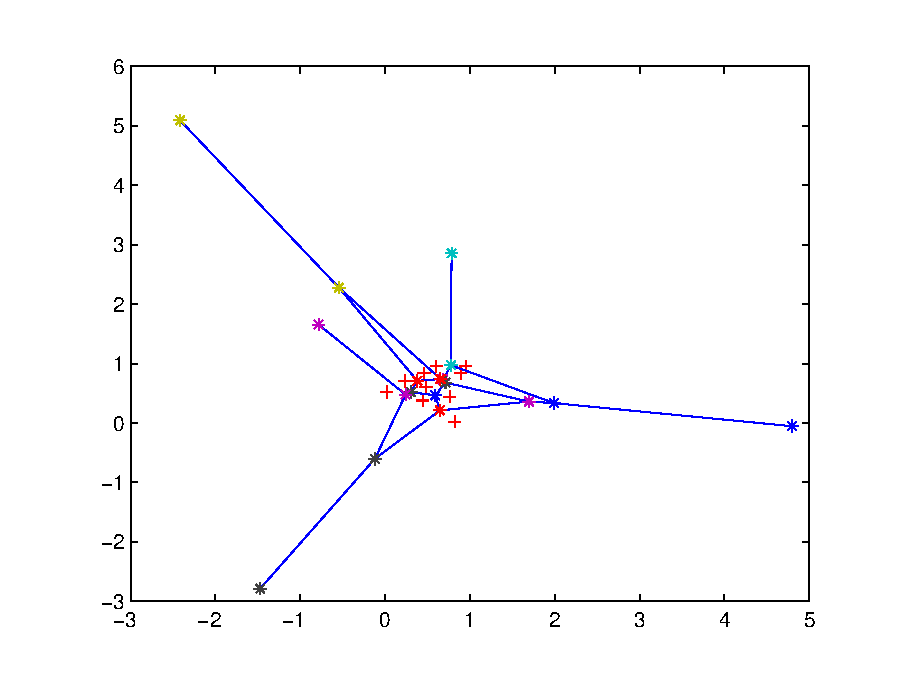
\includegraphics[width=0.3\textwidth,height=0.3\textwidth]{pics/voronoi_0.eps}
	}
\subfigure[]{ 
		\label{fig:subfig:c} %% label for first subfigure 
	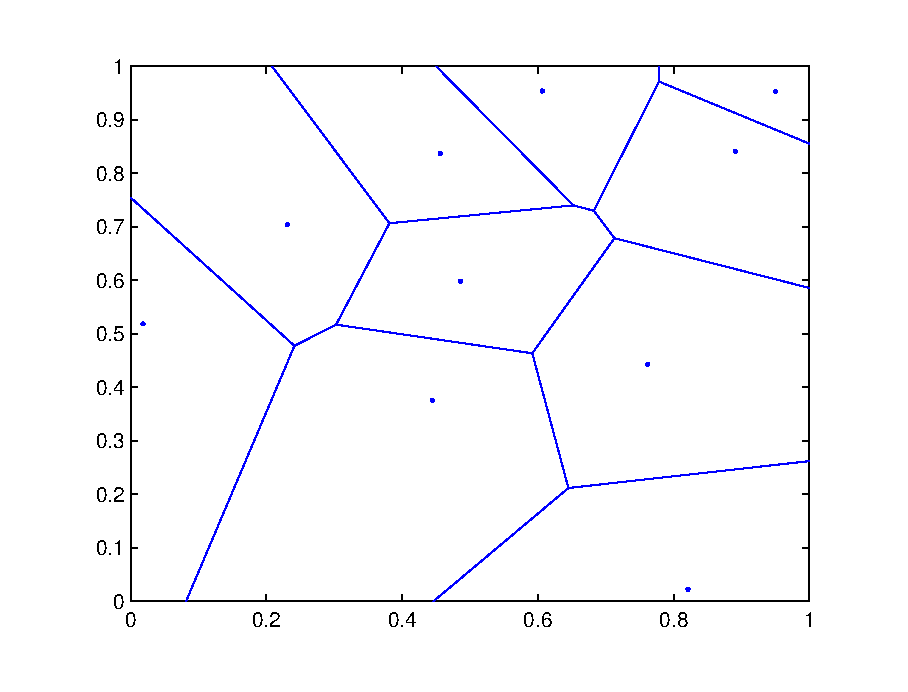
\includegraphics[width=0.3\textwidth,height=0.3\textwidth]{pics/voronoi_1.eps}
	}
\end{center}
	\label{fig:123}
\end{figure}

\begin{figure}[htbp]
	\begin{center}
		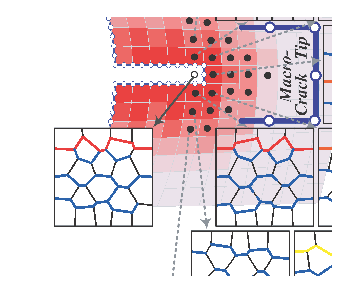
\includegraphics[width=0.3\textwidth]{pics/Micro_structure.eps}
	\end{center}
	\caption{计算中的Voronoi格子}
	\label{fig:vri}
\end{figure}
其中的$b$图是$a$图的局部放大图。可以看出这个才是需要使用的真实计算模型。

\subsection{使用凸包生成软件qhull生成Voronoi图}
qhull包含了一系列的工具,其中qvoronoi就是用来生成Voronoi图的。

软件的输入是一系列的点集
例如
\begin{verbatim}
2
5
0 0.4
1 0
0 1
1 1
0.5 0.5
\end{verbatim}
其中第一行指的是点集的维数,第二行指的是点的数目,以后依次为点的坐标。

输出一般指定为 
\begin{verbatim}
   qvoronoi p Fv
\end{verbatim}

参数$p$表示的是输出点的坐标,$Fv$表示的是输出voronoi边,三维的情形表示的是面。

例如上述点集的输出为
\begin{verbatim}
2
4
0.3666666666666666 -0.1333333333333334 
     1    0.5 
   0.2    0.7 
   0.5      1 
8
4 0 2 0 3
4 0 1 0 1
4 0 4 1 3
4 1 3 0 2
4 1 4 1 2
4 2 3 0 4
4 2 4 3 4
4 3 4 2 4
\end{verbatim}

其中第一行表示的是点集的维数,第二行表示的是有限点的个数,以后四行表示的是有限点的坐标,接下来的一行表示的是voronoi边的个数,接着依次是voronoi边
它里面的数据的表示的是2+Voronoi点数,接下来的两个是输入点编号,并且这两个输入点的中面就是Voronoi边(面),其余的数字表示的是Voronoi边(面)上的Voronoi顶点编号。
注意,其中有限点的编号从1开始,无限点的编号为0,也就是说包含编号0的Voronoi边(面)是开放的。

通常为了处理这样的点,将输出加上Fi选项,即
\begin{verbatim}
   qvoronoi p Fv Fi
\end{verbatim}
输出的结果为

\begin{verbatim}
2
4
0.3666666666666666 -0.1333333333333334 
     1    0.5 
   0.2    0.7 
   0.5      1 
8
4 0 2 0 3
4 0 1 0 1
4 0 4 1 3
4 1 3 0 2
4 1 4 1 2
4 2 3 0 4
4 2 4 3 4
4 3 4 2 4
4
5 0 4 0.9805806756909201 0.196116135138184 -0.3333974297349128 
5 1 4 -0.7071067811865476 0.7071067811865476 0.3535533905932738 
5 2 4 0.7071067811865476 -0.7071067811865475 0.3535533905932737 
5 3 4 -0.7071067811865476 -0.7071067811865476 1.060660171779821
\end{verbatim}

这里的增加了5行为了输出无限点,他们分别表示的是,第一行表示的是包含无限点的面数,其余的为面的信息,
其中第一个数据表示的是该行的数据个数,接下来的两个数表示的是输入点,其余的三个数分别表示的是两个输入点所夹的面的方程系数。
\[Ax+By+C=0\]
或者是
\[
Ax+By+Cz+D=0.
\]

这样就可以用上面生成的数据就可以完整描述一个Voronoi图。

直接读取文件可以使用的qhull的命令行为
\begin{verbatim}
qvoronoi TI test TO file2 p Fv Fi
\end{verbatim}
其中test是输入的文件名,file2为输出的文件名,其余为输出参数。

%\putbib[20120327.sample]             %% list reference.

\newpage
